\documentclass[12pt]{article}
\usepackage[utf8]{inputenc}

\usepackage{amsfonts}
\usepackage{amsmath}
\usepackage{bookmark}
\usepackage[a4paper, margin=3.5cm]{geometry}
\usepackage{graphicx} % For inserting images
\usepackage{hyperref} % For hyperlinks
\usepackage{indentfirst}
\usepackage{minted} % For code-highlighting
\usepackage{parskip}

\graphicspath{ {./images/} }
\setlength{\parindent}{15pt} % Set paragraph indentation
\setlength{\parskip}{1em} % Set paragraph space (one line)
\setminted{frame=single, breaklines} % Set codeblock style

\title{Programming Practicum Report:\\Meeting \#4}
\author{\href{https://github.com/avaxar}{R. Ethan Halim}}
\date{September 16th, 2024}

\begin{document}

\maketitle

\section{Sum of Series}
The entire source file is hosted on a GitHub repository \href{https://github.com/avaxar/uni-practica-1/tree/main/week_4/01_sum}{\textbf{here}}.

\subsection{Explanation}

The program is to compute the sum of an arithmetic series from $1$ to $n$. Firstly, it requests user input for the value of \texttt{n}.

\begin{minted}{cpp}
int program(std::istream& cin, std::ostream& cout) {
    int64_t n;
    cout << "Input: ";
    cin >> n;

    ...
}
\end{minted}

$$\text{val} = \sum_{i = 1}^n i$$

The loop below calculates the sum of the arithmetic series, which is equivalent to the mathematical expression above, and prints the sum.

\begin{minted}{cpp}
int program(std::istream& cin, std::ostream& cout) {
    ...

    int64_t val = 0;
    for (int64_t i = 1; i <= n; i++) {
        val += i;
    }

    cout << "Output: " << val << '\n';

    ...
}
\end{minted}

The explanation to the sum is printed by another loop which at the same time formats the expanded sum of the arithmetic series. The loop iterates from 1 to \texttt{n} and prints them following the printing of \texttt{"(Explanation:"}. In the iterations from 1 to \texttt{n - 1}, \texttt{" + "} is appended to the explanation, as to generate something alike \texttt{"1 + 2 + ... + [n - 1] + [n] = [val]"}.

\begin{minted}{cpp}
int program(std::istream& cin, std::ostream& cout) {
    ...

    cout << "(Explanation: ";
    // If it is equal or below zero, just print "0 = 0".
    if (n <= 0) {
        cout << "0";
    }
    for (int64_t i = 1; i <= n; i++) {
        cout << i;
        if (i != n) {
            cout << " + ";
        }
    }
    cout << " = " << val << ")\n";

    return 0;
}
\end{minted}

\subsection{Manual Testing}
Below is the compilation and the testing of the source code.
\newline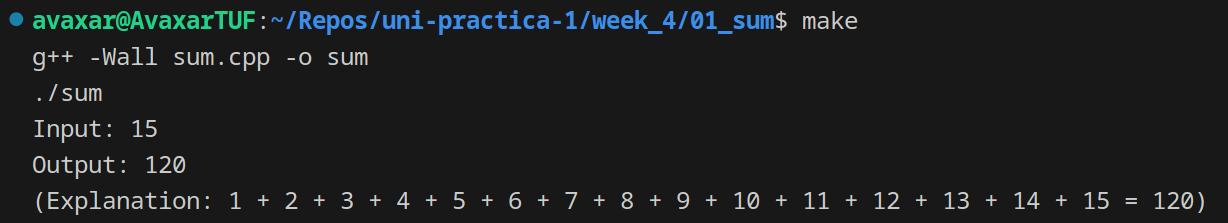
\includegraphics[width=\textwidth]{01_sum}

\subsection{Test Cases}

\subsubsection{Tests}
Below is copied directly from the \texttt{tests.txt} file.
\inputminted{text}{01_sum/tests.txt}

\subsubsection{Execution}
Below are the results of the test cases. No test cases failed.
\newline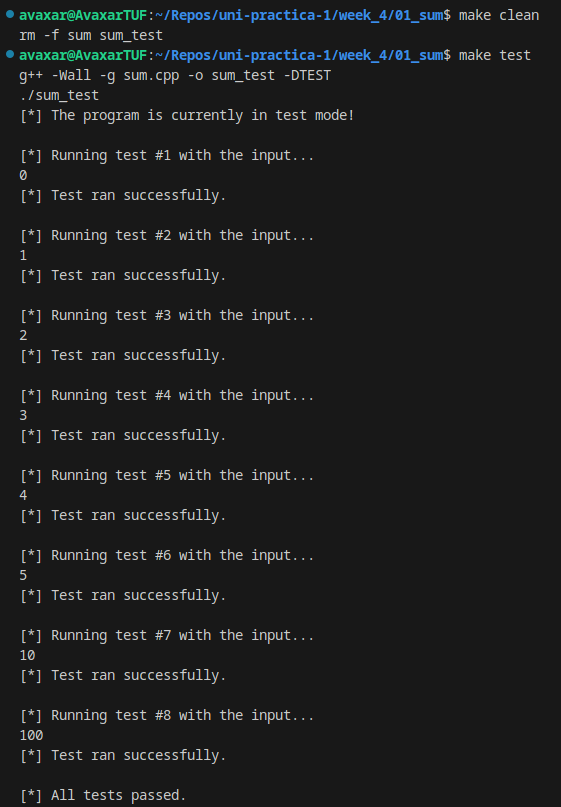
\includegraphics[width=\textwidth]{01_sum_test}

\pagebreak
\section{Multiplication Table}
The entire source file is hosted on a GitHub repository \href{https://github.com/avaxar/uni-practica-1/tree/main/week_4/02_multiplication}{\textbf{here}}.

\subsection{Explanation}

The code iterates from 1 to 10 using a for-loop and multiplies the given input \texttt{n} by the iterator \texttt{i}.

\begin{minted}{cpp}
int program(std::istream& cin, std::ostream& cout) {
    int64_t n;
    cout << "Input: ";
    cin >> n;

    cout << "\n[Multiplication Table]\n";
    for (int64_t i = 1; i <= 10; i++) {
        cout << n << " x " << i << " = " << (n * i) << '\n';
    }

    return 0;
}
\end{minted}

\subsection{Manual Testing}
Below is the compilation and the testing of the source code.
\newline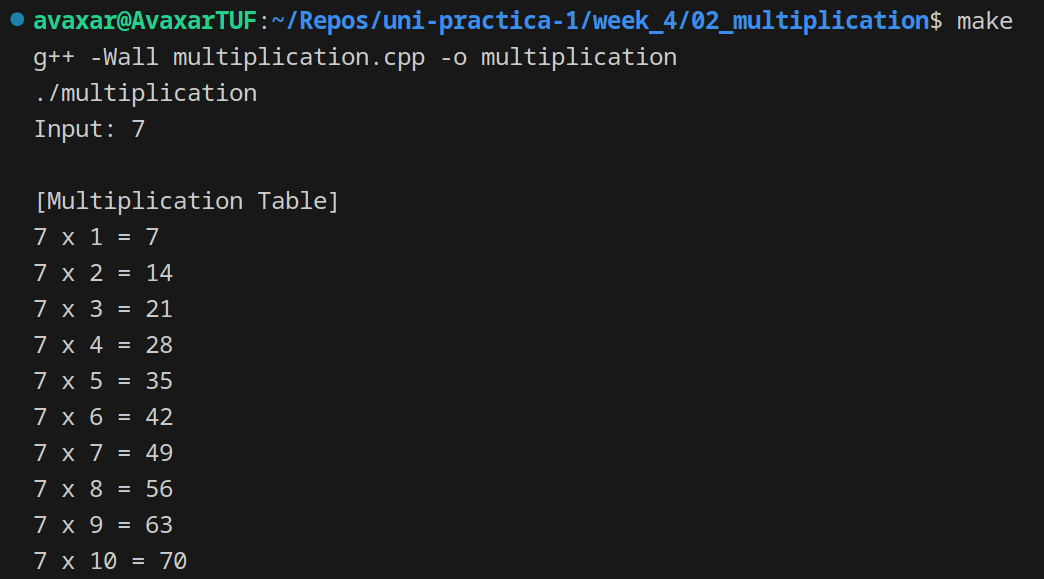
\includegraphics[width=\textwidth]{02_multiplication}

\subsection{Test Cases}

\subsubsection{Tests}
Below is copied directly from the \texttt{tests.txt} file.
\inputminted{text}{02_multiplication/tests.txt}

\subsubsection{Execution}
Below are the results of the test cases. No test cases failed.
\newline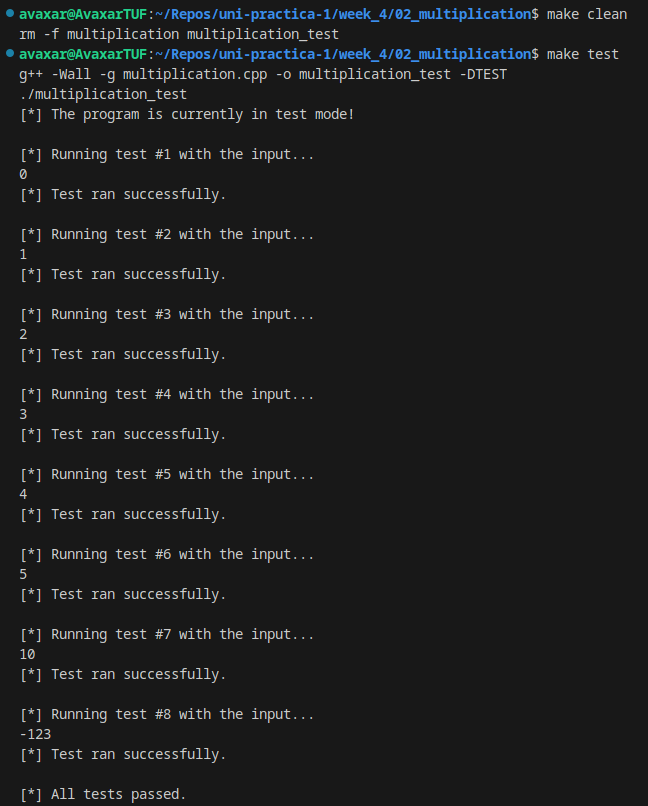
\includegraphics[width=\textwidth]{02_multiplication_test}

\end{document}
